% ============================================================================
% CHAPITRE 3 — ANALYSE DES BESOINS ET CONCEPTION (Part 1: 3.1–3.3)
% ============================================================================

\section{Introduction}

Ce chapitre suit la méthodologie Scrum en présentant les résultats du Sprint 1 consacré à
l'analyse des besoins et à la conception de l'architecture du système. L'objectif est de fournir
une spécification complète et non ambiguë à partir de laquelle les chapitres suivants pourront
implémenter les deux sous-systèmes sans interprétation subjective.

La démarche adoptée progresse en six étapes~: l'identification des acteurs et la modélisation des
cas d'utilisation (section~3.2), l'expression des besoins non fonctionnels (section~3.3),
la conception de l'architecture globale en couches (section~3.4), la spécification du schéma de
base de données (section~3.5), la définition des contrats API REST (section~3.6), et enfin les
considérations de sécurité et de gestion des données (section~3.7).


% ────────────────────────────────────────────────────────────────
\section{Identification des acteurs et besoins fonctionnels}
% ────────────────────────────────────────────────────────────────

\subsection{Identification des acteurs}

Le \textbf{Touriste} constitue l'acteur principal du système. Il peut être anonyme (session sans
authentification) ou identifié (connecté via son compte utilisateur). Le touriste interagit avec
l'interface de chat pour formuler des demandes de planification de voyage, recevoir des itinéraires
structurés, les modifier par des messages de suivi, et consulter l'historique de ses conversations.
Son comportement de navigation --- clics, temps de consultation, profondeur de défilement, ajouts
aux favoris --- est automatiquement capté par le tracker JavaScript pour alimenter le moteur de
recommandation LinUCB.

L'\textbf{Administrateur de la plateforme} est responsable de la supervision technique du système.
Il peut déclencher une reconstruction complète de l'index RAG via l'endpoint
\texttt{POST /admin/rebuild-index} lorsque l'indexation incrémentale se désynchronise, consulter
l'état de santé du système via \texttt{GET /health} (qui vérifie la connexion à la base de données,
la disponibilité d'Ollama si configuré, et l'état de l'index RAG), et sélectionner le fournisseur
LLM par défaut via la configuration du serveur. L'administrateur n'interagit pas directement avec
l'agent conversationnel mais supervise son bon fonctionnement.

Le \textbf{Système} représente l'ensemble des processus automatisés qui s'exécutent sans
intervention humaine. Il comprend les écouteurs d'événements SQLAlchemy qui déclenchent la
réindexation RAG incrémentale lors de modifications en base de données, le tracker JavaScript
qui collecte et transmet les événements comportementaux vers l'endpoint
\texttt{POST /api/recommendations/events}, le planificateur APScheduler qui exécute les trois
jobs nocturnes (mise à jour des profils utilisateur, vérification de la dérive conceptuelle,
rafraîchissement des tags), et la tâche de persistance des matrices LinUCB qui sauvegarde
les matrices A et b en base de données toutes les deux minutes.


\subsection{Diagramme des cas d'utilisation global}

Le diagramme des cas d'utilisation ci-dessous présente une vue d'ensemble des interactions entre
les trois acteurs identifiés et les fonctionnalités principales du système Guidni. Les cas
d'utilisation sont organisés en trois groupes~: les interactions conversationnelles du touriste
avec l'agent planificateur, les opérations d'administration du système, et les processus
automatisés du sous-système de recommandation.

Deux types de relations structurelles enrichissent le diagramme~: la relation d'extension
\texttt{<<extend>>} entre \og{}Modifier un plan existant\fg{} et \og{}Envoyer un message de
planification\fg{} indique que la modification est un cas particulier de l'envoi de message~;
la relation d'inclusion \texttt{<<include>>} entre \og{}Recevoir un plan de voyage\fg{} et
\og{}Valider le plan\fg{} indique que la validation est systématiquement exécutée avant la
présentation du plan au touriste.

\begin{figure}[htbp]
    \centering
    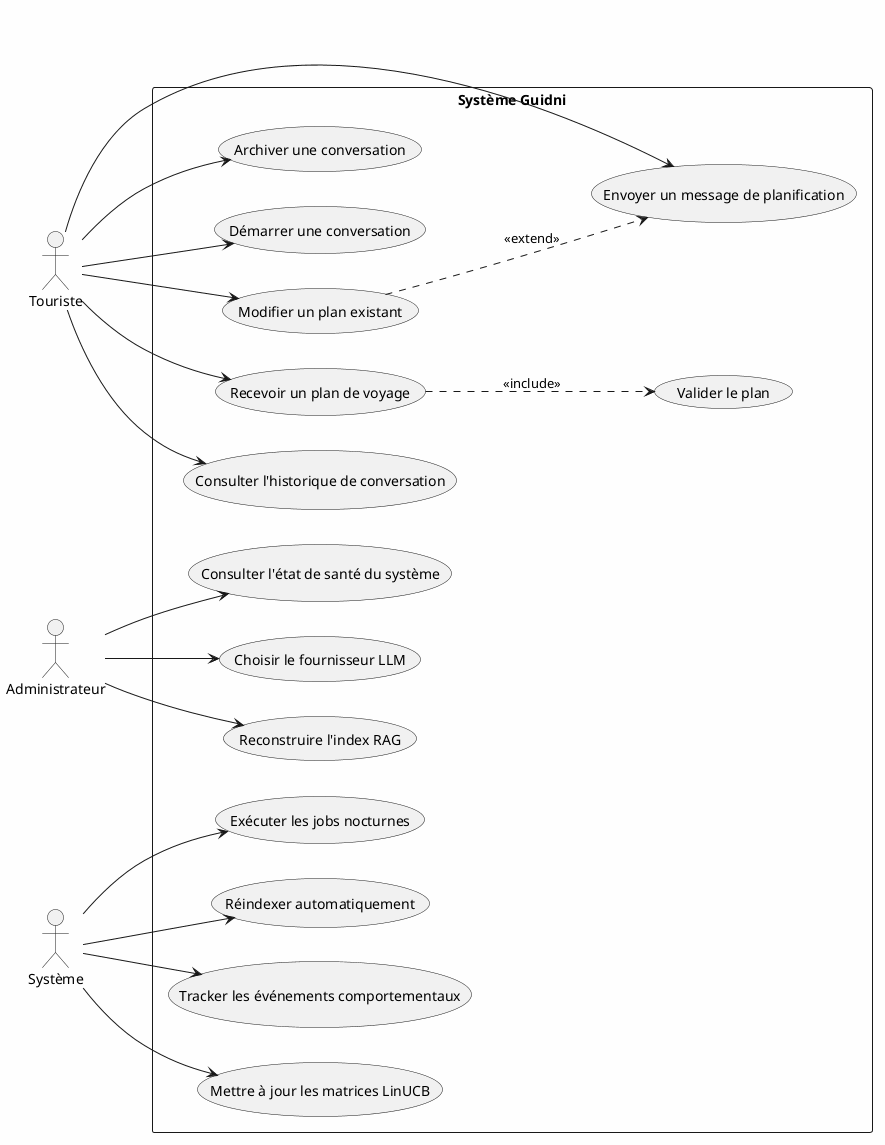
\includegraphics[width=0.9\textwidth]{diagrams/fig_03_use_case_global.png}
    \caption{Diagramme des cas d'utilisation global du système Guidni}
    \label{fig:use_case}
\end{figure}


\subsection{Description détaillée des cas d'utilisation principaux}

Les trois cas d'utilisation les plus critiques du système sont décrits en détail dans les
tableaux suivants. Chaque description spécifie l'acteur déclencheur, les préconditions
nécessaires, le flux principal d'exécution, les flux alternatifs possibles, et les
postconditions garanties.

\begin{table}[htbp]
    \centering
    \caption{UC-01~: Générer un plan de voyage}
    \label{tab:uc01}
    \small
    \begin{tabular}{p{3cm} p{11cm}}
        \toprule
        \textbf{Champ} & \textbf{Description} \\
        \midrule
        Acteur & Touriste \\[3pt]
        Précondition & L'utilisateur existe en base, une conversation est créée ou existante \\[3pt]
        Déclencheur & L'utilisateur envoie un message de planification via \texttt{POST /chat} \\[3pt]
        Flux principal &
        (1) Réception de la requête \texttt{ChatRequest} avec \texttt{user\_id} et \texttt{message} ;
        (2) Validation de l'existence de l'utilisateur en base (HTTP~404 sinon) ;
        (3) Chargement du contexte (8 derniers messages + plan courant + résumé) ;
        (4) Appel de \texttt{run\_agent()} avec le graphe LangGraph ;
        (5) Nœud THINK~: le LLM raisonne avec les 18 outils disponibles ;
        (6) Exécution des outils (recherche RAG, météo, activités, géolocalisation) ;
        (7) \texttt{create\_plan\_structure()} valide le plan contre la base de données ;
        (8) Nœud VALIDATE~: vérification des doublons et du nombre de créneaux ;
        (9) Nœud RESPOND~: sauvegarde du plan dans \texttt{GeneratedPlan} ;
        (10) Retour du \texttt{PlannerResponse} au frontend. \\[3pt]
        Flux alternatif & Le LLM a besoin d'informations $\rightarrow$ outil \texttt{ask\_user} $\rightarrow$
        \texttt{needs\_more\_info=True} $\rightarrow$ RESPOND retourne une question \\[3pt]
        Postcondition & Ligne \texttt{GeneratedPlan} créée, \texttt{PlannerMessage} sauvegardé \\
        \bottomrule
    \end{tabular}
\end{table}

\begin{table}[htbp]
    \centering
    \caption{UC-02~: Obtenir des recommandations personnalisées}
    \label{tab:uc02}
    \small
    \begin{tabular}{p{3cm} p{11cm}}
        \toprule
        \textbf{Champ} & \textbf{Description} \\
        \midrule
        Acteur & Touriste / Système \\[3pt]
        Précondition & Des lignes \texttt{BanditArm} existent pour la zone demandée \\[3pt]
        Déclencheur & Requête \texttt{GET /api/recommendations} avec paramètres de contexte \\[3pt]
        Flux principal &
        (1) Récupération des bras depuis le cache RAM ou la base de données ;
        (2) Chargement du profil utilisateur si \texttt{user\_id} fourni ;
        (3) Construction du \texttt{UserContext} à partir des paramètres de requête ;
        (4) Chargement des matrices A et b depuis le cache RAM ;
        (5) Calcul du vecteur $\phi$ par produit de Kronecker pour chaque bras ;
        (6) Exécution du pipeline de classement en 9~étapes ;
        (7) Retour du \texttt{RecommendationResponse} avec items classés. \\[3pt]
        Postcondition & \texttt{RecommendationEvent} de type \texttt{impression} enregistré \\
        \bottomrule
    \end{tabular}
\end{table}

\begin{table}[htbp]
    \centering
    \caption{UC-03~: Tracker un événement comportemental}
    \label{tab:uc03}
    \small
    \begin{tabular}{p{3cm} p{11cm}}
        \toprule
        \textbf{Champ} & \textbf{Description} \\
        \midrule
        Acteur & Système (tracker JavaScript) \\[3pt]
        Précondition & Session active avec un \texttt{session\_id} valide \\[3pt]
        Déclencheur & L'utilisateur clique, consulte, ou réserve une annonce \\[3pt]
        Flux principal &
        (1) Le tracker JS met l'événement en file d'attente ;
        (2) Toutes les 15~secondes ou tous les 10~événements~: \texttt{flush()} ;
        (3) \texttt{POST /api/recommendations/events} avec le lot d'événements ;
        (4) \texttt{compute\_reward()} calcule la récompense delta pour chaque événement ;
        (5) Le vecteur $\phi$ est calculé pour chaque bras concerné ;
        (6) Les matrices A et b sont mises à jour en RAM ;
        (7) \texttt{log\_event()} et \texttt{update\_arm\_counters()} enregistrent les compteurs ;
        (8) Réponse avec les récompenses de session cumulées. \\[3pt]
        Postcondition & Compteurs \texttt{BanditArm} mis à jour, \texttt{RecommendationEvent} créé \\
        \bottomrule
    \end{tabular}
\end{table}

La section suivante complète l'analyse en spécifiant les besoins non fonctionnels du système.


% ────────────────────────────────────────────────────────────────
\section{Besoins non fonctionnels}
% ────────────────────────────────────────────────────────────────

Les besoins non fonctionnels définissent les contraintes de qualité que le système doit respecter
indépendamment de ses fonctionnalités. Ils sont classifiés selon les catégories de la norme
ISO~25010, qui couvre la performance, la disponibilité, la scalabilité, la maintenabilité, la
sécurité, le support multilingue et la confidentialité des données.

Le tableau suivant synthétise ces besoins avec pour chaque catégorie une mesure cible vérifiable,
permettant de valider le respect de ces exigences lors de la phase de tests présentée au
chapitre~5.

\begin{table}[htbp]
    \centering
    \caption{Besoins non fonctionnels classifiés selon la norme ISO~25010}
    \label{tab:nfr}
    \small
    \begin{tabular}{p{2.5cm} p{5.5cm} p{5.5cm}}
        \toprule
        \textbf{Catégorie} & \textbf{Besoin} & \textbf{Mesure / Cible} \\
        \midrule
        Performance & Latence de l'endpoint \texttt{/chat} & $< 5$\,s (P95) \\
         & Latence \texttt{/api/recommendations} & $< 100$\,ms (P95) \\
         & Scoring LinUCB pour $N=1000$ bras & $< 50$\,ms \\[3pt]
        Disponibilité & Uptime du service & 99,5\% \\
         & Démarrage sans index RAG & Non fatal (mode dégradé) \\[3pt]
        Scalabilité & Pool de connexions psycopg2 & minconn$=2$, maxconn$=10$ \\
         & Pool AsyncPG & pool\_size$=10$, max\_overflow$=20$ \\[3pt]
        Maintenabilité & Ajout d'un nouveau fournisseur LLM & 1 fichier client + config \\
         & Journalisation rotative & 10\,MB info, 50\,MB debug \\[3pt]
        Sécurité & Validation utilisateur & Chaque requête vérifie \texttt{user\_id} \\
         & Limitation de débit événements & 10/listing/session, 100/session \\[3pt]
        Multilingue & Langues supportées & FR, EN, AR (auto-détection) \\
         & Embeddings multilingues & BAAI/bge-m3 (100+ langues) \\[3pt]
        Confidentialité & Données vers LLM externe & Pas de PII sans consentement \\
         & Option locale & Ollama pour souveraineté complète \\
        \bottomrule
    \end{tabular}
\end{table}

La section suivante présente l'architecture globale conçue pour satisfaire ces besoins.


% ────────────────────────────────────────────────────────────────
\section{Architecture globale du système}
% ────────────────────────────────────────────────────────────────

\subsection{Vue d'ensemble architecturale}

Le \textbf{frontend} du système Guidni est une application Next.js couplée à l'ORM Prisma, qui
gère l'interface utilisateur, l'authentification, et les opérations CRUD sur les entités
touristiques (activités, hébergements, restaurants, locations, transferts). Le frontend lit et
écrit dans la base de données PostgreSQL partagée via Prisma, et communique avec le backend IA
via les endpoints REST \texttt{/chat}, \texttt{/plan} et \texttt{/api/recommendations}.

Le \textbf{backend IA} est une application FastAPI qui héberge les deux sous-systèmes
intelligents~: l'agent planificateur LangGraph (9~endpoints REST) et le moteur de recommandation
LinUCB (3~endpoints REST). Il possède en écriture 4~tables planificateur et 7~tables
recommandation, et lit en lecture seule les tables Prisma du frontend. L'application utilise
SQLAlchemy en mode asynchrone avec le pilote asyncpg pour les opérations du planificateur, et
psycopg2 avec un pool de connexions threadé pour les opérations de recommandation en temps réel.

Les \textbf{services externes} comprennent l'API Open-Meteo pour les données météorologiques
en temps réel, le service Nominatim pour le géocodage et le calcul de distances par la formule
de Haversine, le serveur Ollama local pour l'inférence LLM sans réseau, l'API cloud Groq pour
l'inférence rapide, l'API Google Gemini pour les contextes longs, et l'API Lightning AI comme
quatrième fournisseur. Le stockage LlamaIndex sur disque (\texttt{rag\_storage/}) persiste
l'index vectoriel entre les redémarrages.

Le \textbf{tracker JavaScript} est un module vanilla JS sans dépendance externe, intégré dans
les pages du frontend. Il collecte les événements comportementaux (clics, temps de consultation,
défilement, ajout aux favoris, réservations) et les transmet par lots vers l'endpoint
\texttt{POST /api/recommendations/events}. Il utilise l'API \texttt{navigator.sendBeacon()} pour
garantir la transmission des événements même lors de la fermeture de la page.

\begin{figure}[htbp]
    \centering
    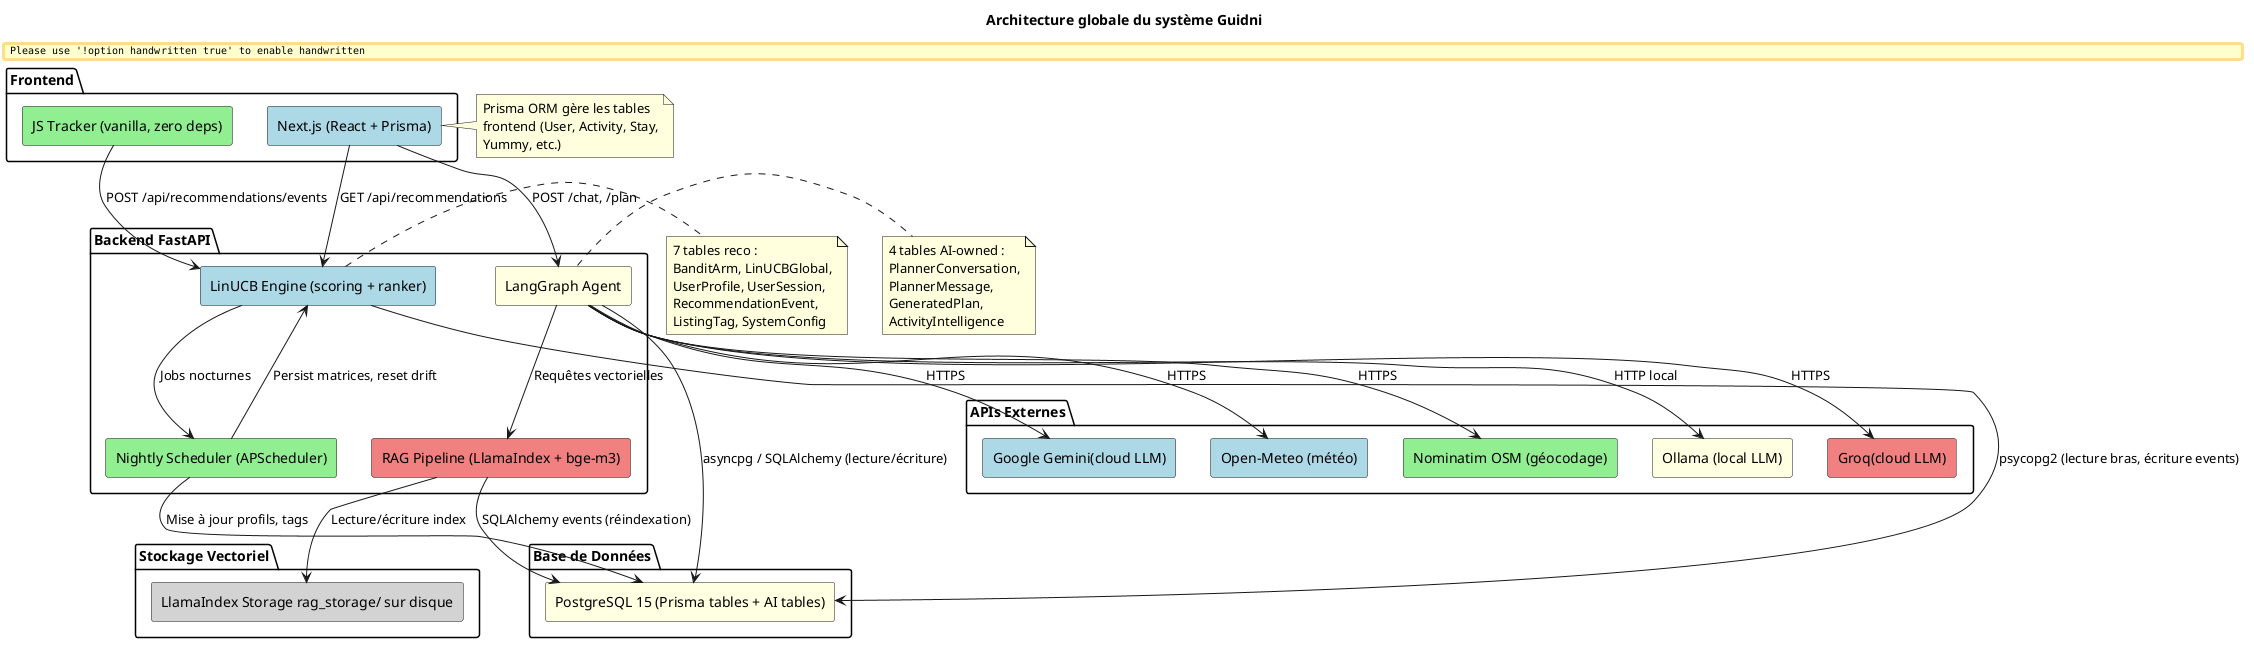
\includegraphics[width=0.9\textwidth]{diagrams/fig_03_global_architecture.png}
    \caption{Architecture globale du système Guidni}
    \label{fig:global_arch}
\end{figure}


\subsection{Architecture en couches}

La \textbf{couche de présentation} comprend les endpoints FastAPI définis dans \texttt{main.py}
et \texttt{recommendation\_router.py}, les schémas Pydantic de requête et de réponse
(\texttt{ChatRequest}, \texttt{PlannerResponse}, \texttt{UserPreferences}), le middleware CORS
configuré pour accepter toutes les origines en développement, et la génération automatique de
documentation OpenAPI accessible via l'endpoint \texttt{/docs}.

La \textbf{couche de logique métier} contient le cœur intelligent du système~: l'agent LangGraph
avec sa machine à états à quatre nœuds et ses 18~outils appelables, le moteur de classement
LinUCB avec son pipeline en 9~étapes, le moteur de requête RAG avec recherche sémantique et
reranking par cross-encoder, et le système de mémoire conversationnelle (chargement des 8~derniers
messages, résumé automatique au seuil de 15~messages, construction du profil utilisateur).

La \textbf{couche d'accès aux données} regroupe les modèles SQLAlchemy ORM et les requêtes
asynchrones pour le sous-système planificateur, le constructeur d'index LlamaIndex avec
persistance sur disque et réindexation incrémentale par événements, et le pool de connexions
psycopg2 (\texttt{ThreadedConnectionPool}, minconn$=2$, maxconn$=10$) pour les opérations de
recommandation en temps réel. La \textbf{couche d'infrastructure} fournit le moteur AsyncPG
avec pool de connexions (pool\_size$=10$, max\_overflow$=20$), le planificateur APScheduler
configuré sur le fuseau horaire Africa/Tunis, la journalisation rotative à deux niveaux
(10~MB info, 50~MB debug), et la gestion de la configuration par variables d'environnement
via \texttt{dotenv}.

La section suivante détaille la conception du schéma de base de données partagé.
% ============================================================================
% CHAPITRE 3 — Part 2: 3.5–3.7 + Conclusion
% ============================================================================

% ────────────────────────────────────────────────────────────────
\section{Conception de la base de données}
% ────────────────────────────────────────────────────────────────

\subsection{Vue d'ensemble du schéma}

Le système Guidni adopte un patron de base de données partagée~: la même instance PostgreSQL~15
est utilisée simultanément par le frontend Next.js/Prisma et par le backend IA FastAPI. Le
backend IA lit 14~tables gérées par Prisma (modèles en lecture seule~: \texttt{User},
\texttt{Activity}, \texttt{Stay}, \texttt{Restaurant}, \texttt{Attraction}, \texttt{Rental},
\texttt{Transfer}, etc.) et possède en écriture 4~tables planificateur et 7~tables
recommandation. Cette architecture évite la duplication des données tout en maintenant des
frontières de propriété claires entre les deux systèmes.

La convention de nommage reflète l'origine de chaque table~: les tables Prisma utilisent le
PascalCase avec guillemets doubles (\texttt{"User"}, \texttt{"Activity"}), les tables
AI-owned du planificateur utilisent également le PascalCase (\texttt{"PlannerConversation"},
\texttt{"GeneratedPlan"}), tandis que les tables de recommandation sont nommées selon les
conventions définies dans le module \texttt{db\_init.py}. Cette distinction visuelle permet
d'identifier immédiatement l'origine et le propriétaire de chaque table.

La stratégie de versionnement des plans repose sur le champ \texttt{isActive} de la table
\texttt{GeneratedPlan}. Lorsqu'un utilisateur modifie un plan existant via un message de suivi,
l'ancien plan est désactivé (\texttt{isActive=False}) et une nouvelle ligne est insérée avec
le champ \texttt{version} incrémenté. Cette approche conserve l'historique complet des plans
générés et permet la récupération de versions antérieures si nécessaire.

\begin{figure}[htbp]
    \centering
    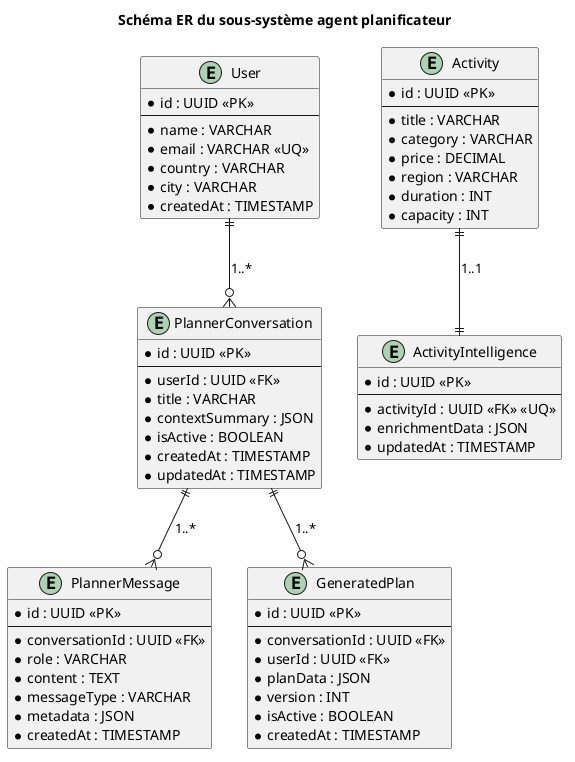
\includegraphics[width=0.85\textwidth]{diagrams/fig_03_er_diagram_planner.png}
    \caption{Schéma ER du sous-système agent planificateur}
    \label{fig:er_planner}
\end{figure}

\begin{figure}[htbp]
    \centering
    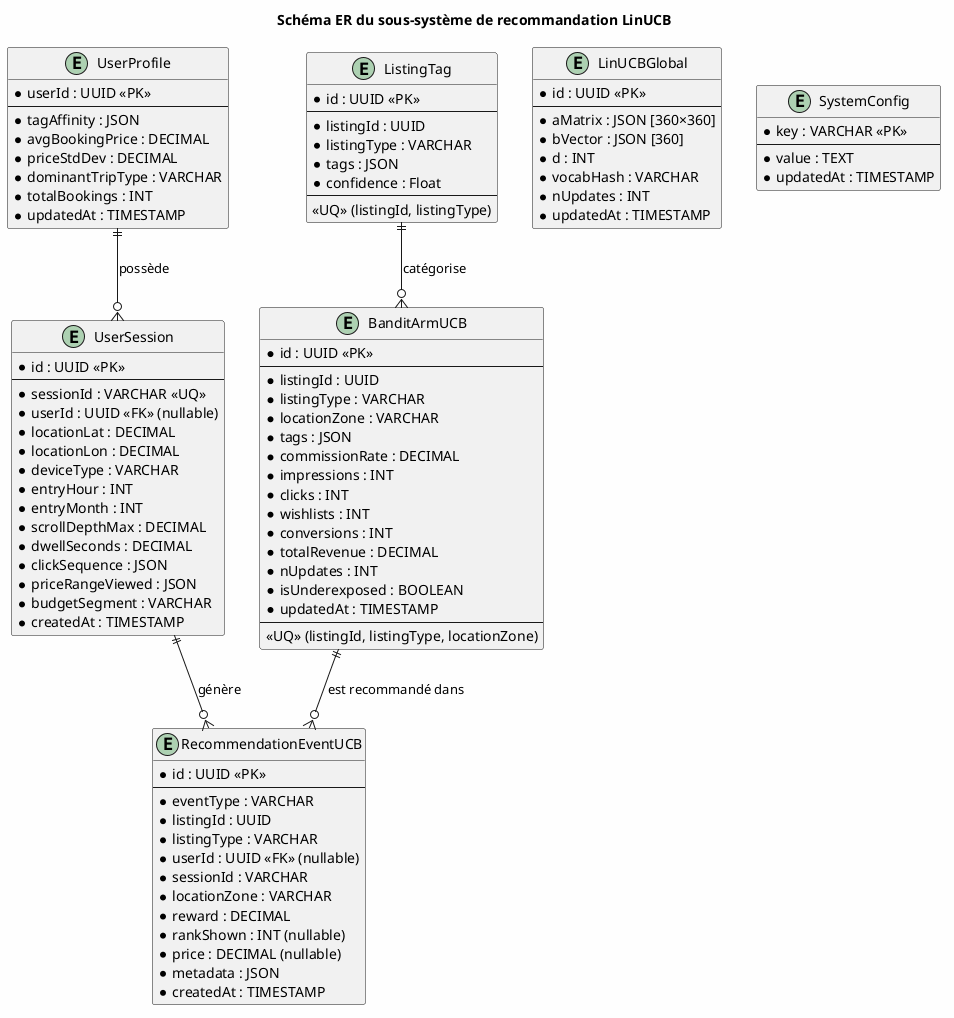
\includegraphics[width=0.9\textwidth]{diagrams/fig_03_er_diagram_recommender.png}
    \caption{Schéma ER du sous-système de recommandation LinUCB}
    \label{fig:er_recommender}
\end{figure}


\subsection{Description des tables clés}

Le tableau suivant récapitule les onze tables détenues par le backend IA, en précisant leur rôle
fonctionnel, les composants qui y écrivent et ceux qui les lisent. Cette matrice de
responsabilité permet de comprendre les flux de données entre les différents composants du
système.

\begin{table}[htbp]
    \centering
    \caption{Description des tables AI-owned}
    \label{tab:ai_tables}
    \small
    \begin{tabular}{p{3.2cm} p{4.5cm} p{2.8cm} p{3cm}}
        \toprule
        \textbf{Table} & \textbf{Rôle} & \textbf{Écrit par} & \textbf{Lu par} \\
        \midrule
        PlannerConversation & Suivi des conversations agent & Agent (main.py) & Agent, Frontend \\[2pt]
        PlannerMessage & Messages individuels & Agent (main.py) & Agent (contexte) \\[2pt]
        GeneratedPlan & Plans versionnés & Agent (RESPOND) & Frontend, Agent \\[2pt]
        ActivityIntelligence & Cache d'enrichissement IA & Agent (outils) & Agent (outils) \\[2pt]
        BanditArm & Compteurs par annonce & Reco router, Nightly & Ranker \\[2pt]
        LinUCBGlobal & Matrices A et b globales & Cache RAM (2~min) & Ranker (scoring) \\[2pt]
        UserProfile & Affinités de tags utilisateur & Job nocturne & Ranker (contexte) \\[2pt]
        UserSession & Données de session navigation & Reco router & Ranker (contexte) \\[2pt]
        RecommendationEvent & Journal des interactions & Reco router & Job nocturne \\[2pt]
        ListingTag & Tags extraits par LLM & Tag extractor & Ranker (phi) \\[2pt]
        SystemConfig & Configuration système & Admin, Nightly & Startup checks \\
        \bottomrule
    \end{tabular}
\end{table}

La section suivante définit les contrats API REST pour les deux sous-systèmes.


% ────────────────────────────────────────────────────────────────
\section{Conception de l'API REST}
% ────────────────────────────────────────────────────────────────

L'API REST du système Guidni suit les conventions RESTful standard~: les méthodes HTTP
(\texttt{GET}, \texttt{POST}, \texttt{DELETE}) correspondent aux opérations de lecture, création
et suppression, les corps de requête et de réponse utilisent le format JSON, et la validation
des entrées est assurée par les schémas Pydantic qui génèrent automatiquement des erreurs~422
en cas de données invalides.

La documentation OpenAPI est générée automatiquement par FastAPI et accessible via l'endpoint
\texttt{/docs}. Elle décrit l'ensemble des endpoints, leurs paramètres, les schémas de requête
et de réponse, et les codes d'erreur possibles. Les deux tableaux suivants spécifient les
contrats API pour chacun des deux sous-systèmes.

\begin{table}[htbp]
    \centering
    \caption{Contrat API --- Sous-système Agent Planificateur}
    \label{tab:api_planner}
    \footnotesize
    \begin{tabular}{p{1cm} p{3.5cm} p{3cm} p{3cm} p{3cm}}
        \toprule
        \textbf{Mét.} & \textbf{Endpoint} & \textbf{Description} & \textbf{Requête} & \textbf{Réponse} \\
        \midrule
        POST & \texttt{/chat} & Chat principal & ChatRequest & PlannerResponse \\[2pt]
        POST & \texttt{/plan} & Pipeline plan & UserPreferences & \{plan\_data\} \\[2pt]
        GET & \texttt{/conversations/ \{user\_id\}} & Lister conversations & --- & \{conversations\} \\[2pt]
        GET & \texttt{/conversations/ detail/\{conv\_id\}} & Détail conversation & --- & \{messages\} \\[2pt]
        DELETE & \texttt{/conversations/ \{conv\_id\}} & Archiver & --- & \{archived\} \\[2pt]
        GET & \texttt{/users} & Lister utilisateurs & --- & \{users\} \\[2pt]
        GET & \texttt{/models} & Modèles LLM & --- & \{models\} \\[2pt]
        POST & \texttt{/admin/ rebuild-index} & Reconstruire RAG & --- & \{documents\_indexed\} \\[2pt]
        GET & \texttt{/health} & État de santé & --- & \{status, db, rag\} \\
        \bottomrule
    \end{tabular}
\end{table}

\begin{table}[htbp]
    \centering
    \caption{Contrat API --- Sous-système de Recommandation}
    \label{tab:api_reco}
    \footnotesize
    \begin{tabular}{p{1cm} p{3.5cm} p{3cm} p{3cm} p{3cm}}
        \toprule
        \textbf{Mét.} & \textbf{Endpoint} & \textbf{Description} & \textbf{Requête} & \textbf{Réponse} \\
        \midrule
        GET & \texttt{/api/ recommendations} & Recommandations & Query params (zone, types, session, hour, month, top\_k) & RecommendationResponse \\[2pt]
        POST & \texttt{/api/ recommendations/ events} & Lot d'événements & BatchRequest (session\_id, events[]) & BatchResponse \\[2pt]
        POST & \texttt{/api/ recommendations/ merge-session} & Fusionner session & \{session\_id, user\_id\} & \{merged\_events\} \\
        \bottomrule
    \end{tabular}
\end{table}


% ────────────────────────────────────────────────────────────────
\section{Sécurité et gestion des données}
% ────────────────────────────────────────────────────────────────

La configuration CORS (\textit{Cross-Origin Resource Sharing}) est définie dans \texttt{main.py}
avec \texttt{allow\_origins=["*"]} pour la phase de développement, permettant au frontend
Next.js de communiquer avec le backend FastAPI sans restriction d'origine. En production, cette
configuration devra être restreinte au domaine spécifique du frontend pour prévenir les
requêtes cross-origin non autorisées.

La validation de l'utilisateur est effectuée sur chaque requête entrante. Avant tout traitement,
le \texttt{user\_id} fourni dans la requête est vérifié par une requête
\texttt{SELECT} sur la table \texttt{"User"}. Si l'utilisateur n'est pas trouvé, une erreur
HTTP~404 est retournée immédiatement avec un message explicite. Cette vérification systématique
empêche tout traitement pour des identifiants inexistants ou forgés.

Le moteur de recommandation implémente une limitation de débit en mémoire pour prévenir les
abus~: un maximum de 10~événements par annonce et par session, et 100~événements au total par
session. Les sessions inactives depuis plus de 2~heures sont automatiquement nettoyées du cache
mémoire pour éviter les fuites de mémoire. Ces seuils sont configurés dans le module
\texttt{recommendation\_router.py} et appliqués avant tout calcul de récompense.

La confidentialité des données est assurée par plusieurs mécanismes~: les résultats des outils
transmis au LLM externe ne contiennent aucune donnée personnelle identifiable (PII) --- seuls
les identifiants, catégories et caractéristiques anonymisées sont envoyés. Le fournisseur Ollama
local offre une option de souveraineté complète pour les déploiements sensibles, car aucune
donnée ne quitte le serveur. Les vecteurs de caractéristiques du moteur LinUCB sont construits
à partir de signaux comportementaux agrégés (profondeur de défilement, temps de consultation)
et non à partir de données personnelles brutes.

\begin{figure}[htbp]
    \centering
    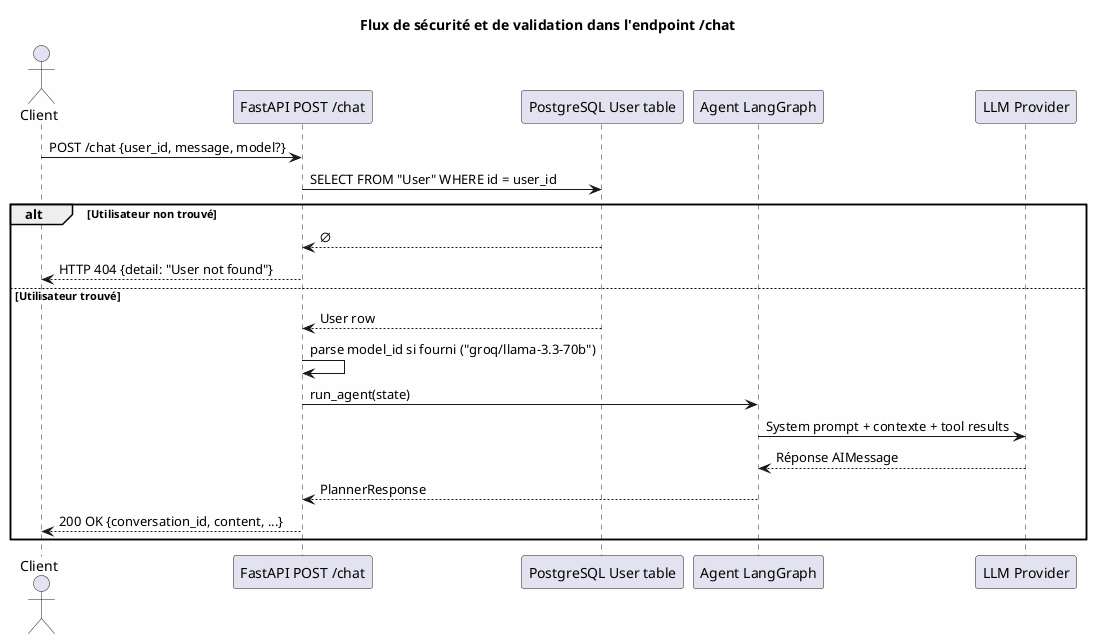
\includegraphics[width=0.85\textwidth]{diagrams/fig_03_security_flow.png}
    \caption{Flux de sécurité et de validation dans l'endpoint /chat}
    \label{fig:security_flow}
\end{figure}


% ────────────────────────────────────────────────────────────────
\section*{Conclusion du chapitre}
\addcontentsline{toc}{section}{Conclusion du chapitre}

Ce chapitre a présenté l'analyse complète des besoins et la conception du système Guidni. Les
trois acteurs du système ont été identifiés (Touriste, Administrateur, Système) et leurs
interactions modélisées par un diagramme de cas d'utilisation global. Les trois cas d'utilisation
principaux ont été décrits en détail~: la génération de plan de voyage, l'obtention de
recommandations personnalisées, et le suivi des événements comportementaux. Les besoins non
fonctionnels ont été classifiés selon la norme ISO~25010, l'architecture globale a été conçue
en couches avec une séparation claire des responsabilités, le schéma de base de données partagé
a été spécifié avec ses 11~tables AI-owned, et les contrats API REST ont été formalisés pour
les 12~endpoints (9~planificateur + 3~recommandation).

Le chapitre suivant présentera l'implémentation détaillée de l'agent planificateur IA, en
décrivant le graphe LangGraph, les 18~outils appelables, le pipeline RAG, et le système de
mémoire conversationnelle.
